\documentclass[tikz,border=3.14mm]{standalone}
\usepackage{pgfplots}
\pgfplotsset{compat=1.17}

\begin{document}
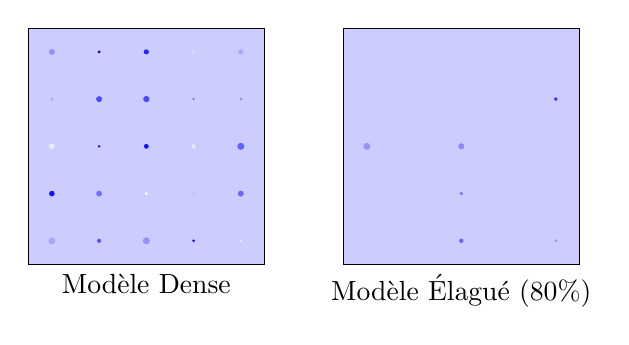
\begin{tikzpicture}

% Dense weights
\begin{scope}[xshift=0cm]
\draw[fill=blue!20] (0,0) rectangle (3,3);
\foreach \x in {0.3,0.9,...,2.7} {
    \foreach \y in {0.3,0.9,...,2.7} {
        \pgfmathsetmacro{\intensity}{rnd*100}
        \pgfmathsetmacro{\size}{0.1 + 0.2*rnd}
        \fill[blue!\intensity] (\x, \y) circle (\size*0.15cm);
    }
}
\node[below] at (1.5,0) {Modèle Dense};
\end{scope}

% Sparse weights
\begin{scope}[xshift=4cm]
\draw[fill=blue!20] (0,0) rectangle (3,3);
\foreach \x in {0.3,0.9,...,2.7} {
    \foreach \y in {0.3,0.9,...,2.7} {
        \pgfmathsetmacro{\rand}{rnd}
        \ifdim \rand pt < 0.2pt % Only 20% of weights remain
            \pgfmathsetmacro{\intensity}{rnd*100}
            \pgfmathsetmacro{\size}{0.1 + 0.2*rnd}
            \fill[blue!\intensity] (\x, \y) circle (\size*0.15cm);
        \fi
    }
}
\node[below] at (1.5,0) {Modèle Élagué (80\%)};
\end{scope}

\end{tikzpicture}
\end{document}